%%% Relatório Técnico - Atividade 4 - UTFPR
%%% Multiplexador Genérico em VHDL

\documentclass[12pt,a4paper, brazil]{article}

%%%%%%% INFORMAÇÕES DO CABEÇALHO
\newcommand{\workingDate}{\textsc{\selectlanguage{portuguese}\today}}
\newcommand{\userName}{LRCO7A}
\newcommand{\institution}{UTFPR-AP}
\usepackage{researchdiary_png}

\usepackage{listings}
\usepackage{float}
\usepackage{placeins}
\usepackage{booktabs}

% Configuração para código VHDL
\lstdefinestyle{vhdl}{
    language=VHDL,
    basicstyle=\ttfamily\small,
    keywordstyle=\color{blue}\bfseries,
    commentstyle=\color{gray}\itshape,
    stringstyle=\color{red},
    numbers=left,
    numberstyle=\tiny\color{gray},
    numbersep=5pt,
    frame=single,
    breaklines=true,
    captionpos=b,
    tabsize=2
}

\begin{document}

\begin{center}
{\textbf {\huge Atividade Prática 4 -- Multiplexador Genérico}}\\[5mm]
{\large Pedro Lucas dos Reis Silva - RA: 2272040} \\[5mm]
{\large Lucas dos Reis Viana - RA: 2321645} \\[5mm]
\today\\[5mm]
\end{center}

% ============================================================
\section{Introdução}
% ============================================================

Esta atividade tem como objetivo a implementação em VHDL de um \textbf{multiplexador genérico} parametrizável tanto no número de entradas quanto na largura de cada entrada. O projeto é validado em duas frentes: uma versão dimensionada para a placa FPGA DE10-Lite (4 entradas de 2 bits, controlada pelas \textit{slide switches}) e uma simulação no Questa Altera Starter FPGA Edition com 16 entradas de 8 bits cada.

Um multiplexador é um circuito combinacional que seleciona uma entre $N$ entradas e a encaminha para a saída, conforme o valor de um sinal de seleção. O número de bits de seleção $S$ relaciona-se com o número de entradas $N$ por
\begin{equation}
    N = 2^S.
\end{equation}
Generalizando, cada entrada pode ter $M$ bits de largura: o mux seleciona o vetor de $M$ bits da entrada apontada por $sel$ e o repete na saída.

Nesta atividade foram introduzidos os seguintes conceitos em VHDL:

\begin{itemize}
    \item \textbf{Estrutura \texttt{generic}}: parâmetros declarados na entidade que são resolvidos em tempo de síntese, permitindo reaproveitar a mesma descrição RTL para várias configurações sem reescrita de código. Os valores reais usados pelo sintetizador são fornecidos no momento da instanciação, via cláusula \texttt{generic map}.
    \item \textbf{Estrutura \texttt{for\ldots generate}}: laço concorrente que replica atribuições e instanciações em tempo de elaboração. A cada iteração, o sintetizador infere uma cópia do hardware descrito no corpo do laço, viabilizando descrições escaláveis em $S$ e $M$.
    \item \textbf{Indexação dinâmica de \texttt{std\_logic\_vector}}: utilização de uma expressão calculada em tempo de execução (no caso, \texttt{to\_integer(unsigned(sel))}) como índice de um vetor, sintetizada como uma rede de multiplexadores.
\end{itemize}

% ============================================================
\section{Desenvolvimento}
% ============================================================

\subsection{Descrição do Problema}

O sistema é dividido em duas entidades VHDL:

\begin{itemize}
    \item \texttt{mux\_generico}: entidade parametrizável que implementa o multiplexador propriamente dito, com generics $S$ e $M$.
    \item \texttt{atividade4}: \textit{top-level} do projeto Quartus, que instancia o \texttt{mux\_generico} com $S=2$ e $M=2$ e conecta as \textit{slide switches} e os displays/LEDs da DE10-Lite.
\end{itemize}

As $N$ entradas são empacotadas em um único \texttt{std\_logic\_vector} de $N \cdot M$ bits, com a entrada $I_0$ ocupando os bits menos significativos. Esse formato evita a necessidade de declarar tipos \textit{array} externos e mantém a interface da entidade dentro dos tipos da biblioteca \texttt{ieee.std\_logic\_1164}. A organização do barramento é
\begin{equation}
    \texttt{entradas}\bigl((i+1)\cdot M - 1 \;\textbf{downto}\; i \cdot M\bigr) \;=\; I_i, \quad i = 0,1,\ldots,N-1.
\end{equation}

\subsection{Implementação do \textit{mux} genérico}

A arquitetura do \texttt{mux\_generico} é puramente concorrente, sem uso de \texttt{process} ou variáveis sequenciais. Para cada bit $j$ da saída ($0 \le j < M$), uma atribuição concorrente conecta \texttt{saida(j)} ao bit $sel \cdot M + j$ do barramento de entradas. As $M$ atribuições são geradas pela estrutura \texttt{for\ldots generate}, conforme apresentado no Apêndice~\ref{ap:codigo-mux}. Cada iteração corresponde, no hardware sintetizado, a um multiplexador $N{:}1$ de 1 bit; os $M$ multiplexadores compartilham o sinal $sel$ e operam em paralelo.

\subsection{Versão na Placa: \textit{Top-level} \texttt{atividade4}}

O \textit{top-level} fixa $S = 2$ e $M = 2$, resultando em $N = 4$ entradas de 2 bits cada. As \textit{slide switches} são distribuídas conforme a Tabela~\ref{tab:mapeamento-sw}.

\begin{table}[H]
\centering
\caption{Mapeamento das \textit{slide switches} -- versão $4{\times}2$ na DE10-Lite.}
\label{tab:mapeamento-sw}
\begin{tabular}{@{}cl@{}}
\toprule
\textbf{Chaves} & \textbf{Função} \\
\midrule
\texttt{sw(1 downto 0)} & entrada $I_0$ (2 bits) \\
\texttt{sw(3 downto 2)} & entrada $I_1$ (2 bits) \\
\texttt{sw(5 downto 4)} & entrada $I_2$ (2 bits) \\
\texttt{sw(7 downto 6)} & entrada $I_3$ (2 bits) \\
\texttt{sw(9 downto 8)} & seleção $sel$ (\texttt{00}--\texttt{11} $\rightarrow$ $I_0$--$I_3$) \\
\bottomrule
\end{tabular}
\end{table}
\FloatBarrier

A saída de 2 bits do mux é enviada simultaneamente aos LEDs e a um decodificador interno de 7~segmentos (função \texttt{dec\_7seg}, herdada da Atividade~3). Os seis displays disponíveis foram aproveitados de modo que o usuário visualize, em tempo real, todas as entradas, a seleção e a saída do mux:

\begin{itemize}
    \item \texttt{HEX0}: saída do mux (entrada selecionada);
    \item \texttt{HEX1}--\texttt{HEX4}: entradas $I_0$, $I_1$, $I_2$, $I_3$;
    \item \texttt{HEX5}: valor da seleção;
    \item \texttt{LEDR(1..0)}: saída do mux em binário;
    \item \texttt{LEDR(9..6)}: ponteiro \textit{one-hot} indicando qual entrada está sendo roteada (gerado por uma atribuição \texttt{with\ldots select}).
\end{itemize}

Mexer em uma chave de uma entrada não selecionada não altera \texttt{HEX0}; mover \texttt{sw(9 downto 8)} faz \texttt{HEX0} saltar para o valor mostrado no display da entrada correspondente.

\subsection{Simulação: \textit{Testbench} 16$\times$8}

Para atender ao item ``\textit{faça uma simulação com um número alto de entradas e de bits de cada entrada}'' do enunciado, foi elaborado o \textit{testbench} \texttt{mux\_generico\_tb}, que instancia o mesmo \texttt{mux\_generico} com $S = 4$ e $M = 8$ ($N = 16$ entradas de 8 bits). Cada entrada é inicializada por um \texttt{for\ldots generate} com o valor $I_i = \texttt{0xA0} + i$, de modo que a saída em hexadecimal segue diretamente o valor de seleção:
\begin{center}
$sel = 0 \rightarrow saida = \texttt{A0}$, \quad $sel = 1 \rightarrow saida = \texttt{A1}$, \quad \ldots, \quad $sel = \texttt{F} \rightarrow saida = \texttt{AF}.$
\end{center}

O processo de estímulo varre as 16 seleções (0 a 15), mantendo cada valor por 20~ns. A simulação foi executada no Questa Altera Starter FPGA Edition acionado a partir do Quartus Prime via \textit{NativeLink} (\textit{Tools} $\rightarrow$ \textit{Run Simulation Tool} $\rightarrow$ \textit{RTL Simulation}). Os sinais \texttt{entradas}, \texttt{sel} e \texttt{saida} foram configurados em radix hexadecimal. A Figura~\ref{fig:simulacao} apresenta o \textit{waveform} resultante, evidenciando a correspondência $sel \leftrightarrow saida$ esperada.

\begin{figure}[H]
    \centering
    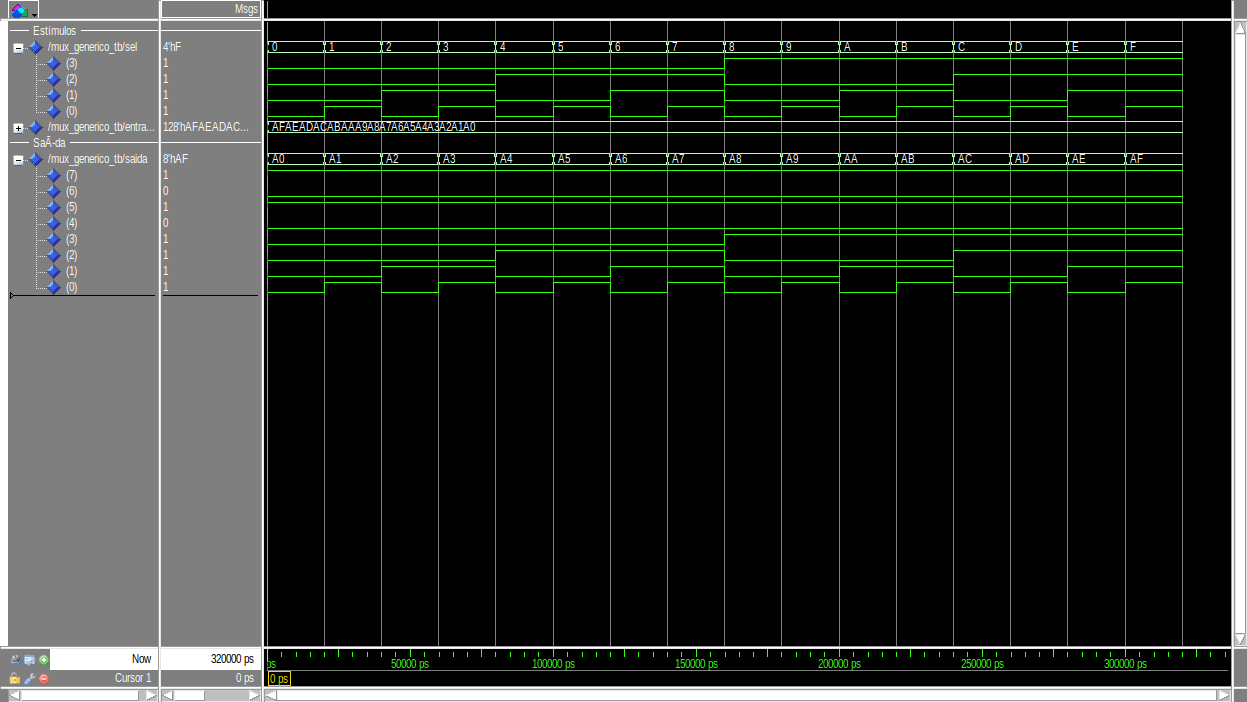
\includegraphics[width=0.95\textwidth]{simulacao_mux.png}
    \caption{\textit{Waveform} da simulação RTL com $S=4$, $M=8$. O sinal \texttt{sel} percorre 0--F e a saída acompanha, retornando os valores 0xA0--0xAF, conforme a tabela do enunciado.}
    \label{fig:simulacao}
\end{figure}
\FloatBarrier

\subsection{Diagrama RTL}

A Figura~\ref{fig:rtl} apresenta o diagrama RTL do \texttt{mux\_generico} (com $S = 2$, $M = 2$) gerado pela ferramenta \textit{Tools $\rightarrow$ Netlist Viewers $\rightarrow$ RTL Viewer} do Quartus Prime. Observa-se a inferência de dois multiplexadores $4{:}1$ -- um para cada bit da saída -- correspondentes às duas iterações do \texttt{for\ldots generate}, ambos compartilhando o sinal $sel$ de 2 bits.

\begin{figure}[H]
    \centering
    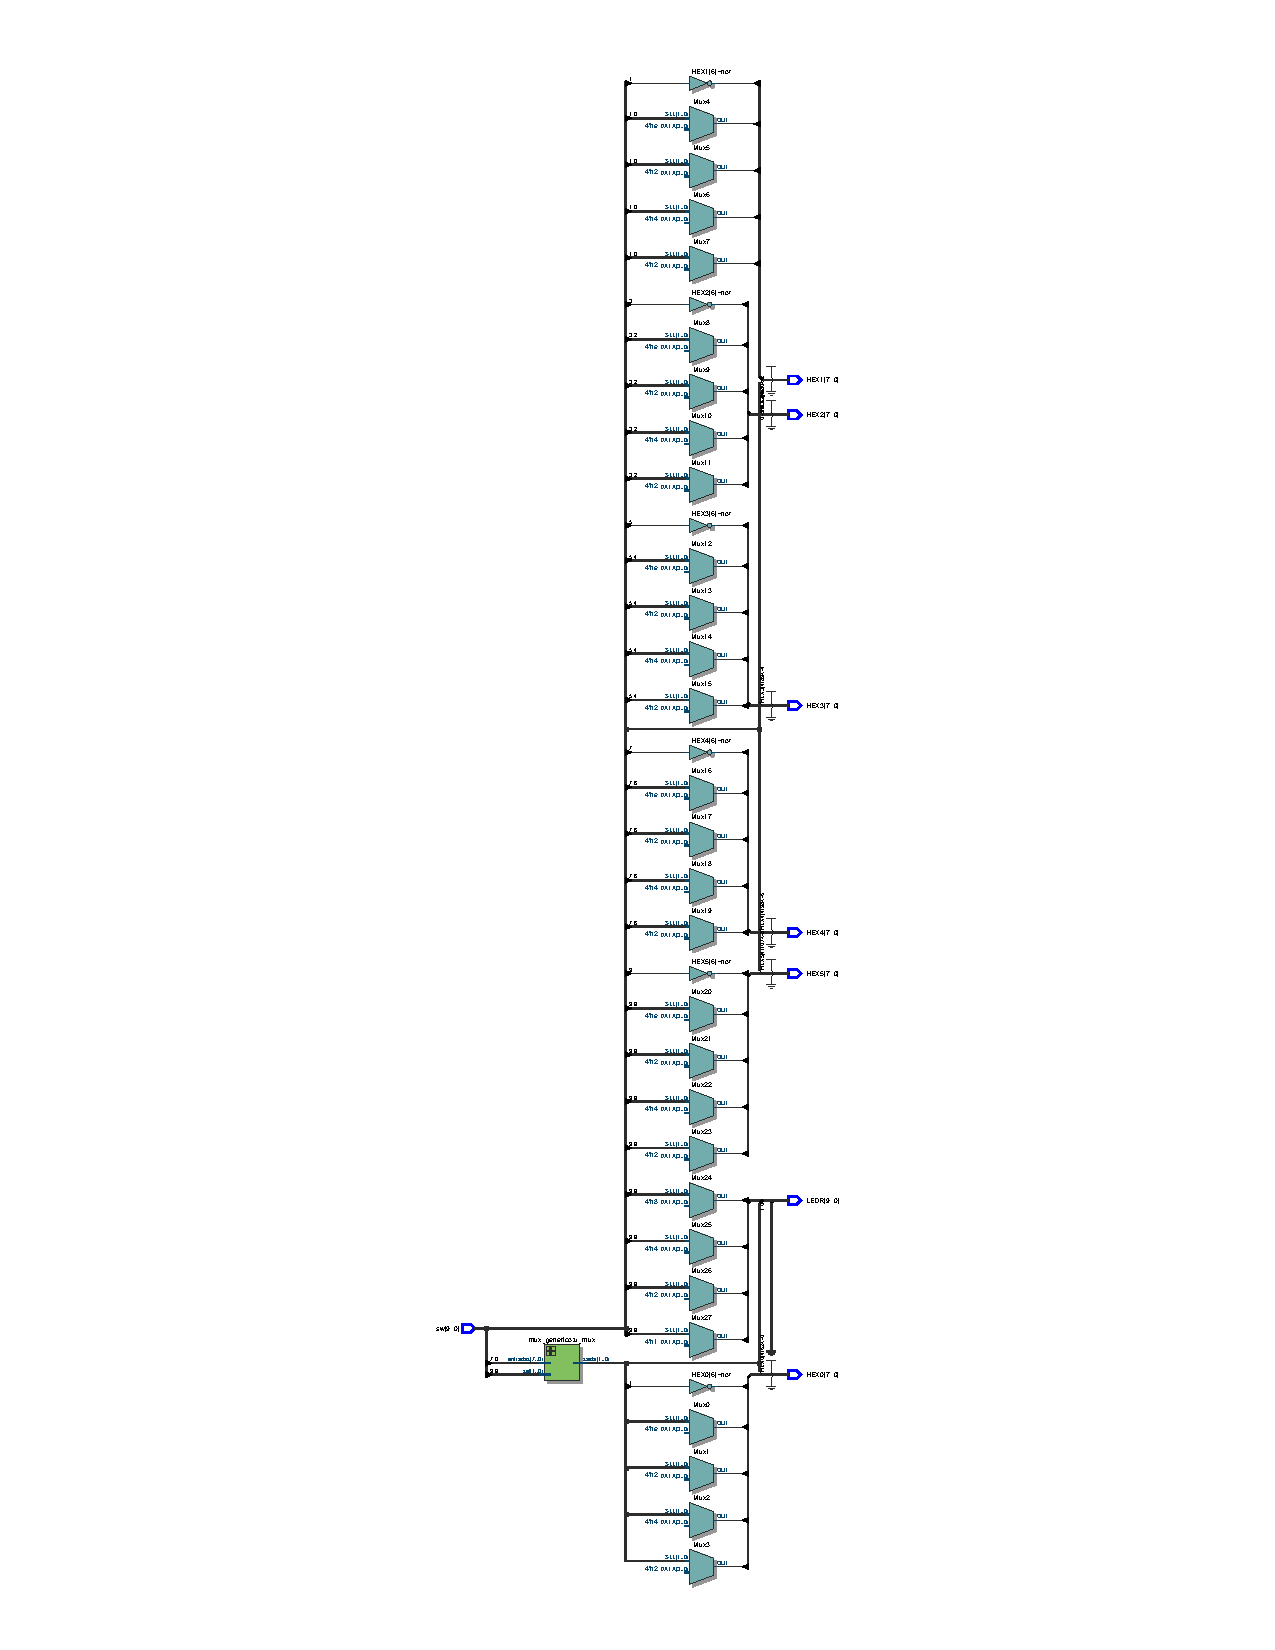
\includegraphics[width=0.95\textwidth]{rtl_mux.pdf}
    \caption{Diagrama RTL do \texttt{mux\_generico} sintetizado pelo Quartus Prime.}
    \label{fig:rtl}
\end{figure}
\FloatBarrier

% ============================================================
\section{Considerações Finais}
% ============================================================

O multiplexador genérico foi implementado com sucesso, atendendo aos itens exigidos pelo enunciado: utilização da estrutura \texttt{generic} com $N$ derivado de $S$ via $N = 2^S$, simulação do projeto com 16 entradas de 8 bits apresentada em hexadecimal, e gravação na placa DE10-Lite da versão de 4 entradas de 2 bits. O uso de \texttt{for\ldots generate} para descrever o corpo do mux permitiu uma arquitetura puramente concorrente -- sem \texttt{process} -- e escalável: trocar os valores de $S$ e $M$ no \texttt{generic map} basta para gerar um mux de qualquer dimensão, sem alterações no código da entidade \texttt{mux\_generico}.

A separação entre a entidade parametrizável (\texttt{mux\_generico.vhd}) e o \textit{top-level} específico da placa (\texttt{atividade4.vhd}) evidencia a distinção entre \textit{generic} -- resolvido em tempo de síntese -- e os dados de entrada propriamente ditos -- amostrados em tempo de execução pelas \textit{slide switches}. A mesma entidade serve tanto à versão sintetizada na FPGA quanto ao \textit{testbench} de simulação, reforçando o ganho de reuso oferecido pela parametrização.

% ============================================================
\appendix
% ============================================================

\newpage
\section{Código VHDL -- Multiplexador Genérico}
\label{ap:codigo-mux}

\begin{lstlisting}[style=vhdl, caption={Arquivo \texttt{mux\_generico.vhd} -- entidade parametrizável.}]
library ieee;
use ieee.std_logic_1164.all;
use ieee.numeric_std.all;

entity mux_generico is
    generic (
        S : positive := 2;
        M : positive := 2
    );
    port (
        entradas : in  std_logic_vector(M*(2**S)-1 downto 0);
        sel      : in  std_logic_vector(S-1 downto 0);
        saida    : out std_logic_vector(M-1 downto 0)
    );
end entity mux_generico;

architecture comportamental of mux_generico is
begin

    -- Para cada bit j da saida, liga ao bit (sel*M + j) do
    -- barramento de entradas. O for...generate cria M atribuicoes
    -- concorrentes; cada uma sintetiza como um mux N:1 de 1 bit.
    gen_bits : for j in 0 to M-1 generate
        saida(j) <= entradas(to_integer(unsigned(sel)) * M + j);
    end generate;

end architecture comportamental;
\end{lstlisting}

\newpage
\section{Código VHDL -- \textit{Top-level} \texttt{atividade4}}
\label{ap:codigo-top}

\begin{lstlisting}[style=vhdl, caption={Arquivo \texttt{atividade4.vhd} -- instancia o mux com $S=2$, $M=2$ e mapeia as chaves, displays e LEDs da DE10-Lite.}]
library ieee;
use ieee.std_logic_1164.all;

entity atividade4 is
    port (
        sw   : in  std_logic_vector(9 downto 0);
        HEX0 : out std_logic_vector(7 downto 0);
        HEX1 : out std_logic_vector(7 downto 0);
        HEX2 : out std_logic_vector(7 downto 0);
        HEX3 : out std_logic_vector(7 downto 0);
        HEX4 : out std_logic_vector(7 downto 0);
        HEX5 : out std_logic_vector(7 downto 0);
        LEDR : out std_logic_vector(9 downto 0)
    );
end entity atividade4;

architecture rtl of atividade4 is

    -- Decodificador 2 bits -> 7 segmentos (anodo comum, formato
    -- DP g f e d c b a; DP fixo em '1'/apagado).
    function dec_7seg(v : std_logic_vector(1 downto 0))
        return std_logic_vector is
    begin
        case v is
            when "00"   => return "11000000"; -- 0
            when "01"   => return "11111001"; -- 1
            when "10"   => return "10100100"; -- 2
            when "11"   => return "10110000"; -- 3
            when others => return "10000110"; -- E
        end case;
    end function;

    constant S : positive := 2;
    constant M : positive := 2;
    constant N : positive := 2**S;

    signal entradas  : std_logic_vector(M*N - 1 downto 0);
    signal saida_mux : std_logic_vector(M - 1 downto 0);

begin

    entradas <= sw(M*N - 1 downto 0);

    u_mux : entity work.mux_generico
        generic map (
            S => S,
            M => M
        )
        port map (
            entradas => entradas,
            sel      => sw(9 downto 9 - S + 1),
            saida    => saida_mux
        );

    HEX0 <= dec_7seg(saida_mux);          -- saida do mux
    HEX1 <= dec_7seg(sw(1 downto 0));     -- I0
    HEX2 <= dec_7seg(sw(3 downto 2));     -- I1
    HEX3 <= dec_7seg(sw(5 downto 4));     -- I2
    HEX4 <= dec_7seg(sw(7 downto 6));     -- I3
    HEX5 <= dec_7seg(sw(9 downto 8));     -- selecao

    LEDR(1 downto 0) <= saida_mux;
    LEDR(5 downto 2) <= (others => '0');

    with sw(9 downto 8) select
        LEDR(9 downto 6) <= "0001" when "00",
                            "0010" when "01",
                            "0100" when "10",
                            "1000" when "11",
                            "0000" when others;

end architecture rtl;
\end{lstlisting}

\newpage
\section{Código VHDL -- \textit{Testbench}}
\label{ap:codigo-tb}

\begin{lstlisting}[style=vhdl, caption={Arquivo \texttt{mux\_generico\_tb.vhd} -- simulação com $S=4$, $M=8$ (16 entradas de 8 bits).}]
library ieee;
use ieee.std_logic_1164.all;
use ieee.numeric_std.all;

entity mux_generico_tb is
end entity mux_generico_tb;

architecture sim of mux_generico_tb is

    constant S : positive := 4;
    constant M : positive := 8;
    constant N : positive := 2**S;

    signal entradas : std_logic_vector(M*N - 1 downto 0);
    signal sel      : std_logic_vector(S - 1 downto 0);
    signal saida    : std_logic_vector(M - 1 downto 0);

begin

    DUT : entity work.mux_generico
        generic map (
            S => S,
            M => M
        )
        port map (
            entradas => entradas,
            sel      => sel,
            saida    => saida
        );

    -- Inicializa cada entrada com I_i = 0xA0 + i
    gen_entradas : for i in 0 to N-1 generate
        entradas((i+1)*M - 1 downto i*M)
            <= std_logic_vector(to_unsigned(16#A0# + i, M));
    end generate;

    -- Varre todas as 16 selecoes, mantendo cada uma por 20 ns.
    estimulo : process
    begin
        for i in 0 to N-1 loop
            sel <= std_logic_vector(to_unsigned(i, S));
            wait for 20 ns;
        end loop;
        wait;
    end process;

end architecture sim;
\end{lstlisting}

\end{document}
